\documentclass[12pt]{article}

% links
\usepackage[colorlinks]{hyperref}
\hypersetup{allcolors=blue}
\usepackage[capitalise]{cleveref}
\usepackage{mathptmx}

% sections
% section and subsection titles
\usepackage{titlesec}
\titlespacing*{\section}
{0pt}{1.5\baselineskip}{2\baselineskip}
\titlespacing*{\subsection}
{0pt}{1.5\baselineskip}{\baselineskip}
\titleformat{\section}
{\normalfont\Large\bfseries}{\thesection}{1em}{}
\titleformat{\subsection}
{\normalfont\large\bfseries}{\thesubsection}{1em}{}
%{0pt}{5.5ex plus 1ex minus .2ex}{4.3ex plus .2ex}
% section and subsection numbering
\renewcommand{\thesubsection}{\Alph{subsection}.}
\renewcommand{\thesection}{\Roman{section}.}
% indent after subsection
\usepackage{indentfirst}

% column margins
\usepackage[margin={1.5cm,1.5cm}]{geometry} 
%\setlength{\columnsep}{.5cm}

% multicolumns 
%\usepackage{multicol, caption} 

% images and captions
\usepackage{wrapfig}
\usepackage{graphicx}
\usepackage[export]{adjustbox} % allows alignment of figures
\usepackage{floatrow} % allows captions to the side
\usepackage{caption} 
\captionsetup{font=footnotesize}

%citation
\usepackage[round, authoryear]{natbib}
\bibliographystyle{abbrvnat}
\usepackage[colorlinks,citecolor=blue,urlcolor=blue,bookmarks=false,hypertexnames=true] {hyperref} 

%custom
\newcommand\thesistitle{Rate and persistence of adaptation remains consistent across multiple sets of spectral cues for sound localisation}

% title
\newenvironment{sc_figure} % single column figure environment
  {\par\medskip\noindent\minipage{\linewidth}}
  {\endminipage\par\medskip}



\begin{document}

\title{\thesistitle}% title page 
\author{Paul Friedrich\\Department of Biology, Leipzig University}
\date{February 2023}
\maketitle

Accurate localization of sounds is required for navigation, communication, predation and escape. It is therefore not surprising that neural and structural specializations have evolved to perform this complex task. The human cortex for example continuously integrates sensory input across modalities to estimate the relative direction and distance of objects (things) in the environment. Whereas the topography of visual and somatosensory space is represented by a point‐by‐point mapping of primary receptors, the auditory scene must first be computed from incoming sound waves. In this scenario, the direction-dependent filtering profile of the pinnae and upper body result in spectral cues that aid in the inference of sound source location.As these filters underlie lifelong changes, beyond the developmental period, the auditory system must maintain its ability to recalibrate the mapping of spectral cues to locations in space. [source] 


\section{METHODS}\label{sec2}%Methods
\subsection{Participants}
15 participants (11 females and 4 males) took part in the experiment.
They were informed about the relevant experimental procedures before providing their consent. Participants had no history of hearing disorder and had normal or corrected vision. The experimental procedures were approved by the ethics committee at Leipzig University. Monetary compensation was provided to the participants based on the time they spend at the experiment.

\subsection{Earmolds}
To alter participants’ perception of sound source elevation, their pinnae were consecutively modified by two sets of silicone molds. As a result, spectral cues derived from the shape of the external ears were changed sufficiently to diminish participants ability to locate sounds on the vertical axis. Earmolds were created by applying fast curing, skin safe silicone (SkinTite, Smooth-On, Macungie, USA) to the cymba conchae, cavum conchae and the antihelix while keeping the ear canal unobstructed [Fig. X]. Shape and volume of the earmolds varied between individuals to achieve similar degrees of disruption of vertical sound localization across participants. Two participants did not complete the experiment (first earmolds: n = 14, second earmolds: n = 13) and were removed from the analysis for these molds. 

\subsection{Experimental procedure}
The experiment was designed to adapt listeners to multiple sets of spectral cues for sound localization. Participants wore two distinct pairs of earmolds consecutively (further denoted as molds 1 and molds 2), each over the course of a five-day adaptation period. The acoustical and behavioral impact of the molds were measured and the trajectories of participants’ adaptation throughout the following days were recorded to capture the occurrence of metaplasticity. To test whether learning a new set of spectral cues interferes with a previously learned mapping, the persistence of adaptation to the initial earmolds was measured after participants adapted to the second pair of molds for five days. This measurement was repeated for the second set of molds after five days without earmolds (see \cref{fig:adaptation}). During their first visit, participants were familiarized with the environment, equipment and procedures of the free-field localization task. To minimize procedural learning during the experiment, participants completed at least one localization run and were free to continue practicing until they felt comfortable with the task. No feedback was given. After the initial familiarization, participants performed one localization task to measure their baseline localization accuracy. Once this task was completed, participants’ DTFs were \newpage
\begin{wrapfigure}[15]{l}{4cm}
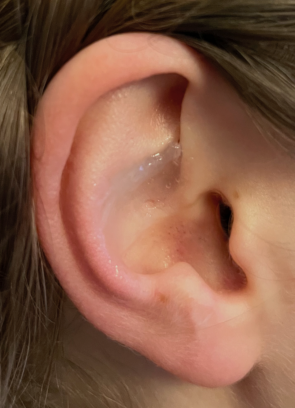
\includegraphics[width=4cm]{../Results/figures/earmold/mold}
\caption{Example of a silicone mold in the right ear of a participant.}
\label{fig:earmold}
\end{wrapfigure}
\noindent\vspace{0\baselineskip}
acquired. Participants’ ears were then modified by fitting the first pair of earmolds, before immediately repeating the localization task. To capture changes to spectral cues induced by the earmolds, DTFs were measured again with the molds in place. From that day on, the first set of silicone molds were worn by the participants for five consecutive days. Throughout this adaptation period, participants underwent a daily routine of training sessions. Each training session was followed by a free-field localization task. On the final day of the first adaptation period (day 5 in \cref{fig:adaptation}), participants completed a short training session and a localization test. As a control, a subset of 6 participants performed an additional localization task presenting stimuli with varying spectral content (USOs) in each trial. The earmolds were then removed, and participants’ localization accuracy was immediately measured again to test for aftereffects of the adaptation. The second pair of earmolds was then fitted to the participants’ ears, their initial localization accuracy was measured and DTFs were acquired. Over the next 5 days, the procedure was repeated as described for the first adaptation period, including daily training sessions and localization tasks. After mold removal at the end of the second adaptation period (day 10 in \cref{fig:adaptation}), the first set of earmolds was briefly re-inserted and participants completed a localization run. To compare the persistence of adaptation to both sets of molds, participants returned to the lab after 5 days for a final localization test with the second molds re-inserted. The localization tests, binaural recordings and training sessions were conducted in a hemi-anechoic room (a x b x c m). Participants were seated in a comfortable chair in front of a spheric array of 45 loudspeakers (Mod1, Orb Audio, New York, USA) with a radius of 1.4 m, covering the frontal hemisphere. Loudspeakers were hidden by an acoustically transparent curtain to avoid visual cues of the sound source positions. Optionally, a small light emitting diode that was visible through the curtain indicating the center of the frontal hemifield (0° Azimuth, 0° Elevation). During the localization tasks and training sessions, participants wore a headband with a laser pointer and an electromagnetic motion sensor (METAMOTIONRL, MBIENTLAB INC, San Francisco, USA) attached. The laser light was reflected by the curtain and provided visual feedback for the participants to indicate  sound source direction by pointing their head at the perceived location. Real time head orientation and position captured by the motion sensor were used to calculate azimuth and elevation of participants’ responses.

\subsection{Stimuli}
The stimuli used in the free-field localization task were 225 ms long sequences of pulsed pink noise, each composed of five equally spaced bursts of 25 ms duration. In the additional localization task, stimuli consisted of 225 ms long mixtures of environmental sounds (USOs). Each stimulus in this test was composed of 6 randomly arranged excerpts of sounds drawn from a list of 42 recordings and had a unique spectrum.Stimuli were re-generated for each trial and controlled by the slab toolbox \citep{schonwiesner_soundlab_2021} in a custom python script. Overall sound pressure level (SPL) of the stimuli at the position of the participants’ ears was 42 dB. Stimuli were processed digitally and amplified via TDT System 3 hardware (Tucker Davis Technologies, Alachua, USA). To minimize spectral localization cues independent of participant’s DTFs, transfer functions for every loudspeaker were measured by a probe microphone (Brüel \& Kjær, Nærum, Denmark) positioned at equal distance and orientation. A bank of inverse finite impulse response filters was designed for each speaker to reduce differences in amplitude and frequency response across the loudspeakers. 

\subsection{Localization task} 
44 Loudspeakers were used for the localization task, covering 102° in azimuth (-52.5° to 52.5°) and 75° in elevation (-37.5° to 37-5°) of the hemisphere in front of the participant. Loudspeaker positions are described in an interaural-polar coordinate system. The loudspeakers were arranged on a spherical grid, formed by 7 loudspeakers on the horizontal and 7 loudspeakers on the vertical axis. Loudspeakers were distributed on the sphere with an angular distance of 17.5° in azimuth and 12.5° in elevation between neighboring speakers. The central and the four outermost loudspeakers (at $\pm$- 52.5° azimuth and  $\pm$ 37.5° elevation) were excluded. At the beginning of each trial, participants were instructed to aim the head mounted laser at a centrally presented LED while pressing the button on a handheld box. When the button was pressed, participant’s initial head position was recorded and the stimulus was presented at a pseudorandom direction. Participants were instructed to indicate the perceived direction by turning their head towards the sound source and to confirm their response by pressing the button again. The horizontal and vertical angular displacement from the initial to the indicating head orientation was used to measure participant’s responses. No feedback was given. Each direction was presented three times during a localization run, with an angular distance of at least 35° between sound locations of two consecutive trials to reduce adaptation and assimilation \citep{ward_stimulus_1979}. 

\subsection{Training}
The training task, inspired by the one described in \citet{trapeau_fast_2016}, was designed to accelerate the adaptation to new spectral cues and was introduced to participants as a game-like scenario. They were instructed to find the location of a pulsed pink noise played from one of the 44 speakers. Proprioceptive feedback was provided by varying pulse duration and the delay between the pulses depending on participant’s head orientation. Duration and delay of consecutive pulses decreased logarithmically with the angular distance between sound direction and the listeners head direction, from up to 500 ms at 65° angular distance. The pulse train gradually merged into a continuous sound when participants directed the head mounted laser within 3° angular distance to the sound source. If participants remained oriented at the target area for at least 500 ms, the sound source was considered found and a popular video game sound was played as a reward signal. The target sound location was then switched at least 45° away from the previous location. Additionally, participants scored points for every found location and were rewarded more points if they located the sounds faster. Participants tried to score as many points as possible within 90 seconds. The final score was displayed on a screen after each round and a leaderboard encouraged a sportive competition. Throughout the adaptation periods, participants underwent a daily routine of three 10-minute training sessions, intermitted by 5-minute breaks.



\subsection{Directional transfer functions}
Binaural recordings were conducted to extract directional transfer functions (DTFs) of participant’s pinnae with and without silicone molds. PUM-3046L-R miniature microphones (PUIaudio, Fairborn, USA) were inserted in the ear canal to measure the sound pressure level at the ear eardrum. To minimize non-directional contributions by standing-wave pattern in the canal, the microphones were placed 2 mm into the entrance of the blocked ear canal. Participants were seated in front of the loudspeaker array and were asked to remain stationary during the measurement while aiming the head mounted laser at the central LED. Frequency modulated sweeps of 100 ms duration were presented 30 times from each of the 7 loudspeakers on the vertical midline (from -37.5° to 37.5° elevation, at 0° azimuth). Recordings were averaged for every location to increase signal to noise ratio. Recordings were digitized via TDT system 3 hardware at a sampling rate of 97 kHz. DTFs were extracted from the time-averaged recordings by taking the ratio of the Fourier transform of the acquired signal to the Fourier transform of the input signal. To reduce non-directional portions of the transfer functions (such as ear canal resonance and mi-\newpage
\begin{wrapfigure}[16]{r}{10cm}
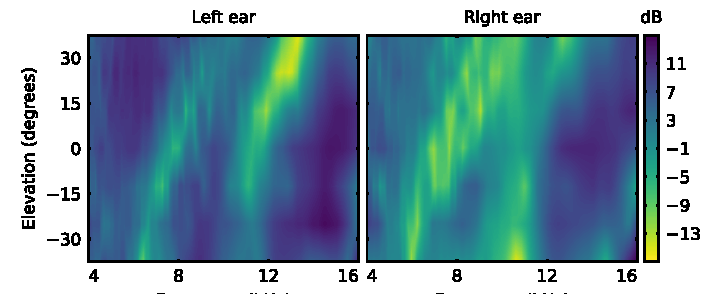
\includegraphics[width=10cm]{../Results/figures/fig1/fig1}
\caption{DTFs across 7 elevations on the vertical midline obtained from one participant. Color maps show the spectral amplitude computed at 83 frequency bins between 4 and 16 kHz. The spectral profile was linearly interpolated between the measured DTFs for display.}
\label{fig:ef_l_r}
\end{wrapfigure}
\noindent
crophone transfer function) each measured transfer function was divided by the grand average across all DTFs of all participants with and without molds (n = 588). To avoid over-representing higher frequencies, DTFs were processed with a bank of octave spaced cosine band-pass filters as proposed by \citet{middlebrooks_individual_1999}. Center frequencies were equally spaced at 0.0286 octaves between 4 and 16 kHz resulting in 2\% frequency difference between each of the 83 filters. The DTFs obtained from the left and right ear of one participant are shown in \cref{fig:ef_l_r}. Spectral information in participants' DTFs that could potentially guide vertical sound localization was quantified by vertical spectral information (VSI) and spectral strength. Vertical spectral information (VSI) was previously defined by \citet{trapeau_fast_2016} as one minus the mean of the coefficients obtained from the autocorrelation matrix of a set of DTFs, i.e., the matrix of correlation coefficients between the DTFs of each elevation against each other \citep{hofman_spectro-temporal_1998}. Spectral strength was defined as the variance of each DTF, averaged across elevations \citep{andeol_sound_2013}. Acoustic dissimilarity between successive pinna shapes (free ears, earmolds 1 and earmolds 2) was quantified by VSI dissimilarity \citet{trapeau_fast_2016}, and was defined as the root-mean-square distance between the correlation matrix of two sets of DTFs and the autocorrelation matrix of the DTFs measured with free ears. VSI, VSI dissimilarity and spectral strength were computed from DTFs obtained from the left and right ear. For comparison with behavioral measures left and right ear values were averaged.

\subsection{Statistical analysis}
Sound localization accuracy was quantified by the root mean square of the distance (RMSE) between the physical target and the perceived response locations for azimuth and elevation respectively. Horizontal and vertical variance of participant’s responses was quantified by taking the grand mean across standard deviations (SD) of the response coordinates for each sound location. Participant’s ability to perceive sound source elevation was additionally quantified by the elevation gain (EG), as the slope of the linear regression lines between target and response elevations \citep{hofman_relearning_1998}. Throughout the analysis, paired comparisons were statistically assessed using Wilcoxon signed-rank tests. Relations between measures were determined using Spearman correlation coefficients, p-values smaller than 0.05 were regarded as significant.


% effects of Pinna-modification

\noindent \textbf{Earmolds reduced spectral information available for vertical sound localization}\\
Application of silicone molds to the Pinnae altered spectral cues across the 4-16 kHz band (Fig. 1, A-C). Both sets of earmolds attenuated the prominent spectral notch situated in the 5-12 kHz band and neighbouring spectral peaks. Similar effects have been observed in previous studies using molds to modify spectral cues \citep{trapeau_fast_2016}\citep{wanrooij_relearning_2005}\citep{hofman_relearning_1998}. Vertical spectral information and spectral strength was computed in 5 octave bands between 4 and 16 kHz (4–8 kHz, 4.8–9.5 kHz, 5.7–11.3 kHz, 6.7–13.5kHz, 8–16kHz) from sets of DTFs obtained with and without Earmolds. As previously reported by \citet{trapeau_fast_2016}, VSIs of participants’ free ears varied among frequency bands (Kruskal-Wallis test, p = 8x10-3) and peaked in the 5.7 – 11.3 kHz band (Fig 2 A). Comparing vertical spectral information in this band to participants' localization performance a correlation with the vertical variance of participants' responses was found (Spearman correlation of free ears VSI and vertical SD: R = - 0.55, p = 0.031). No correlation existed between VSI or spectral strength  in this band and the other behavioral metrics. \citet{middlebrooks_individual_1999} reported a systematic variation in the frequencies of spectral features among individuals’ DTFs within the 3.7 – 12.9 kHz band. To account for the inter-individual differences in the distribution of spectral information across octave bands in the present data (see SE / errorbars in Fig. 2 A) behavioral measures were additionally compared to spectral features in a wider range of frequencies. Here the relation between participants’ free ears VSI and vertical localization accuracy was in the predicted direction, although not significant (Fig 2 B, Spearman correlation of free ears VSI and vertical RMSE: R = - 0.39, p = 0.151). The comparison between VSIs of modified ears and participants’ free ears showed a reduction of vertical spectral information available for elevation discrimination in the 5.3-11.7 kHz octave band (one-tailed Wilcoxon signed rank test; VSI free ears: 0.61 +/- 0.04, VSI earmolds 1: 0.45 +/- 0.05, p = 0.003, VSI earmolds 2: 0.39 +/- 0.04, p = 0.004). The VSI of the left and right ear without molds were correlated in this band as expected (Spearman correlation of left ear and right ear VSI; R = 0.55, p = 0.035). This correlation persisted after application of earmolds  but was not significant for the second set of molds (earmolds 1: R = 0.56, p = 0.035, earmolds 2: R = 0.53, p = 0.064). Figure 2 C shows the VSI of all participants with free ears and both sets of earmolds.\\

\end{multicols} %%% figure 1 A B C: DTFs of free vs modified ears 
\begin{figure}[hb]
\floatbox[{\capbeside\thisfloatsetup{capbesideposition={right,top},capbesidewidth=4cm}}]{figure}[\FBwidth]
{\caption{A test figure with its caption side by side}\label{fig:test}}
{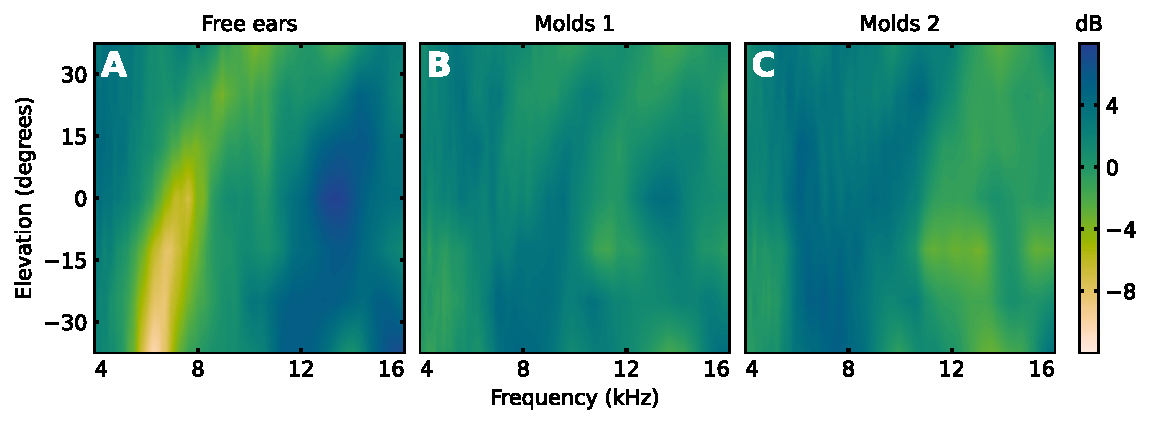
\includegraphics[width=14cm]{../Results/figures/hrtf_compare/hrtf_compare}}
\end{figure}
\begin{multicols}{2}
\noindent % prevent indent

%%% figure 2:  A: free ears VSI across bands, B: correlation free ears VSI and baseline localization accuracy, C: VSI of left and right ear across participants and conditions

\noindent\textbf{Modified pinna shapes were within the physiological range}\\
To confirm that spectral changes induced by the earmolds were physiologically plausible, the VSI dissimilarities in the 5.7-11.3 kHz band between the free and modified ears of each participant were compared to VSI dissimilarities between all possible pairs of participants’ free ears [Fig 4 B]. The overlap of distributions shows that spectral changes induced by both sets of molds were comparable in magnitude to the natural spectrum of differences between individuals’ ears.\\

\noindent\textbf{Spectral changes occurred at similar frequencies across participants and were different for both sets of earmolds}\\
To confirm whether spectral changes occurred at similar frequencies across participants yet were at different frequencies for the two consecutive sets of earmolds, the probability of spectral change between free ears and earmolds was mapped for each frequency bin and elevation (Fig. 3 A-C). Spectral changes were defined as the absolute differences between DTFs measured before and after mold insertion above a given threshold. This threshold was a participant-specific measure of spectral difference across DTFs with free ears and was defined by the mean RMS difference across all combinations of DTFs (in dB) at each elevation (average across participants: 4.89 dB +/-0.15). Based on these thresholds, binary maps of spectral changes were created for each set of earmolds and participant (above-threshold changes were set to 1, all other values were set to 0). The average of these maps across participants shows the proportion of participants for which earmolds induced spectral changes above the threshold at each frequency bin and elevation.\\

\end{multicols} %%% figure 1 D E F spectral change probability 
\begin{figure}[hb]
\floatbox[{\capbeside\thisfloatsetup{capbesideposition={left,top},capbesidewidth=5cm}}]{figure}[\FBwidth]
{\caption{A test figure with its caption side by side}\label{fig:test}}
{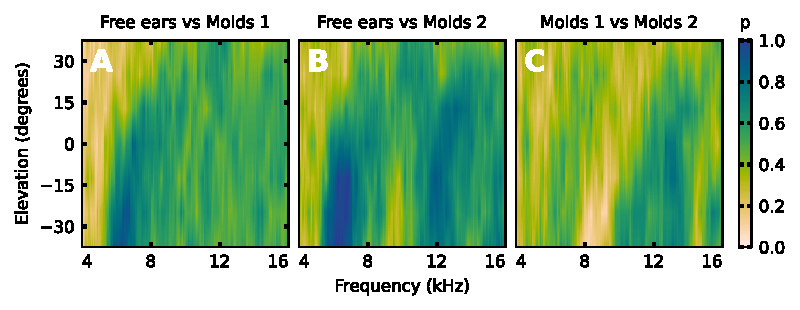
\includegraphics[width=13cm]{../Results/figures/spectral_change_p/spectral_change_p}}
\end{figure}
\begin{multicols}{2}
\noindent % prevent indent


%%%%%% Behavior %%%%%%%
\noindent \textbf{Earmolds reduced vertical localization performance}\\
Insertion of earmolds degraded vertical localization performance (see Fig. 1, days 0 and 5; one-tailed Wilcoxon signed rank test of localization performance; ears free vs earmolds 1; EG: p = 3x10-5, RMSE: p = 3x10-5, SD: p = 6x10-3, ears free vs earmolds 2; EG: p = 5x10-4, RMSE: p = 5x10-4, SD: p = 5x10-4). On the horizontal plane, only the standard deviation of responses increased (one-tailed Wilcoxon signed rank test of performance; ears free vs earmolds 1; SD: p = 0.04, ears free vs earmolds 2: SD: p = 5x10-3). Both sets of earmolds caused a similar decrease of vertical localization performance (two-tailed Wilcoxon signed rank test, differences between free ears and earmolds 1 on day 0 vs difference between ears free and earmolds 2 on day 5; EG: p = 0.465, RMSE: p = 0.700, SD: p = 0.123).\\ %\vfill\null\columnbreak 
 
 \noindent\textbf{Participants consecutively adapted to two novel sets of DTFs}\\
Participants wore two different sets of earmolds during two consecutive 6-day adaptation periods. Adaptation was driven by multisensory experience while wearing the molds throughout the day, accompanied by five sessions of daily sensory-motor training at the lab. Vertical sound localization performance improved significantly for both sets of earmolds except for response variability (SD), which increased throughout the adaptation period (Fig 1, one-tailed Wilcoxon signed rank tests of first vs last day of molds; Earmolds 1: EG: p = 3x10-5, RMSE: p = 6x10-5, SD: p = 0.008; Earmolds 2: EG: p = 3x10-4, RMSE: p = 0.032, SD: p = 0.004). As expected, horizontal localization was not affected by adaptation to the earmolds (Fig 3 B, one-tailed Wilcoxon signed rank tests of first vs last day of molds; Earmolds 1; RMSE: p = 0.555, SD: p = 0.467; Earmolds 2; RMSE: p = 0.485, SD: p = 0.515).\\

\end{multicols} %%% figure 2
\begin{figure}[hb]
\floatbox[{\capbeside\thisfloatsetup{capbesideposition={left,top},capbesidewidth=5cm}}]{figure}[\FBwidth]
{\caption{A test figure with its caption side by side}\label{fig:test}}
{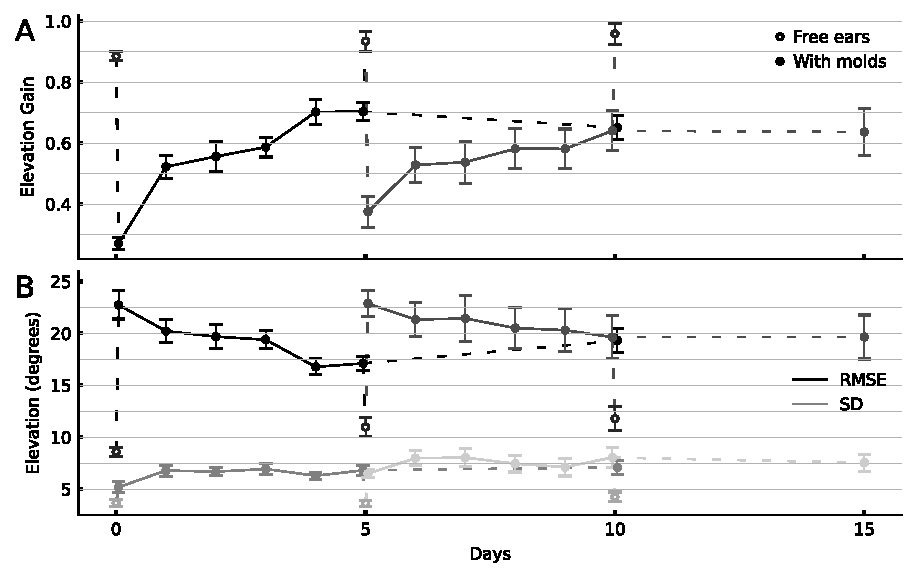
\includegraphics[width=13cm]{../Results/figures/ele_learning/ele_learning}}
\end{figure}
\begin{multicols}{2}
\noindent % prevent indent

\noindent \textbf{No difference between rates of adaptation to first and second earmolds}\\
To investigate possible effects of metaplasticity (i.e., an effect of the previous adaptation to earmolds 1 on the subsequent adaptation to earmolds 2) the rates of adaptation to the first and second earmolds were compared. To assess the rate of adaptation across participants independent of initial acoustical disruption caused by the earmolds, the increase in vertical localization accuracy during adaptation (performance on day 0 vs day 6) was divided by the initial decrease caused by the molds. Individual adaptation rates varied continuously and did not fall into discernable groups. No difference was found between the two sets of earmolds (two-tailed Wilcoxon signed rank test of Molds 1 vs Molds 2, Reduction of vertical RMSE from day 0 to day 6 divided by initial increase; Earmolds 1: 0.66 +/- 0.06 vs Earmolds 2:  0.74 +/- 0.09, p = 0.413). Individual adaptation performance with the first set of earmolds was positively related to adaptation performance with the second set of molds, although not significant (R = 0.47, p = 0.142). No correlation was found between vertical spectral information of the earmolds in the 3.7 – 12.9 kHz band and adaptation performance.\\

\noindent\textbf{Adaptation was generalizable}\\
To rule out the possibility of participants memorizing location-specific spectral features of the training stimuli in the localization test, the test was repeated with a subset of six participants on the last day of each adaptation period using stimuli of random spectral content (USOs). The effect of USO stimuli on vertical localization error did not differ between adapted earmolds and free ears indicating that generalizable perceptual learning had taken place (Friedman test; differences in vertical RMSE between pink noise and USO localization across conditions; Ears free: -0.38 +/- 1.82, Earmolds 1: 2.5 +/- 0.46, Earmolds 2: -0.15 +/- 0.45, p = 0.135).\\

\noindent\textbf{No aftereffect on free ears localization performance after mold removal}\\
Previous studies reported the absence of an aftereffect on localization performance with free ears after adaptation to new spectral cues for sound localization (Hofman 1998, Trapeu and Schönwiesner 2015). To confirm these findings, free ears localization accuracy was measured immediately after mold removal at the end of each adaptation period. 
No aftereffect was present for elevation gain but. An increasing impact on participants’ vertical localization accuracy with their native ears was observed after each adaptation period (see Fig. 1 B, one-tailed Wilcoxon signed rank test, vertical RMSE; free ears baseline vs free ears day 5: p = 0.002, free ears baseline vs free ears day 10: p = 6x10-4). \\



%%%%% spectral behavior %%%%%%%


\noindent\textbf{Differences between first and second mold VSI dissimilarity to free ears}\\
Silicone molds were fitted with the aim of achieving consistent reduction of vertical localization performance across subjects and earmolds. To achieve this, stronger alterations in morphological features of the outer ears became necessary for the second set of molds compared to the first set. Consequently, differences between DTFs with molds and participants’ free ears were larger for the second set of earmolds (Wilcoxon one tailed signed rank test, VSI dissimilarity in the 3.7 – 12.9 kHz band, ears free and earmolds 1:  0.56 +/- 0.06 vs ears free and earmolds 2: 0.72 +/- 0.07, p = 0.002).\\

\noindent\textbf{Effects of acoustic dissimilarity between free ears and earmolds on localization accuracy}\\
To investigate whether acoustic and behavioral effects of the earmolds were related, the VSI dissimilarity between DTFs in the 3.7 – 12.9 kHz band with and without molds was compared to the decrease in participant’s localization performance after insertion of the earmolds. A trend of increasing vertical RMSE for larger acoustic differences was found for the first set of earmolds (Fig 5 B, Spearman correlation of vertical RMSE in the first test with molds compared to free ears and VSI dissimilarity: R = 0.38, p = 0.175). The relation between acoustic differences and behavior was still visible on the last day of the adaptation period (Fig 5 C, Spearman correlation of vertical RMSE in the last test with molds compared to free ears baseline and VSI dissimilarity: R = 0.38, p = 0.185). No such trend was found for vertical localization and VSI dissimilarity between free ears and the second set of molds (Spearman correlation of vertical RMSE in the first test with molds compared to free ears baseline and VSI dissimilarity: R = - 0.07, p = 0.832). Because initial vertical localization accuracy with the second earmolds could additionally depend on acoustic similarities to the previously learned set, differences in localization performance between the final test with earmolds 1 and the initial test with the earmolds 2 were compared to the VSI dissimilarity between both molds. A trend was found of increasing vertical error with greater acoustic dissimilarity between the first and second set of earmolds (Fig 5 D, Spearman correlation of vertical RMSE in the first test with second molds compared to last test with first molds and VSI dissimilarity: R = 0.29, p = 0.385).\\


\section{Discussion}\label{sec1}%Introduction

Listeners were successively adapted to distinct sets of spectral cues for sound localization to investigate effects of metaplasticity and interference between the learned spectral mappings. Modified pinna shapes were sufficiently different to cause repeated disruption of vertical localization. Participants relearned sound localization with both sets of silicone molds within consecutive five-day adaptation periods. Individual adaptation performance did not improve with the second set, suggesting an absence of meta-plasticity. Adaptation persistence did not differ between earmolds, showing that learning a second set of modified spectral cues does not degrade the previously learned representation. In contrast to previous findings, adaptation to new spectral cues reduced participants vertical accuracy with free ears.

%\subsection{Acoustic comparison of the successive earmolds}
\subsection{Acoustic comparison of pinna modifications}

Application of silicone molds modified participants DTFs in a wide range of frequencies (see \cref{fig:spectral_change}) and resulted in large behavioral effects. This study aimed to compare the effects of learning multiple sets of spectral cues on adaptation rate and persistence. To enable this comparison, the magnitude of acoustic changes caused by the two sets of earmolds should be similar. It has been shown that larger acoustic differences between free and modified ears caused a stronger decrease in vertical localization performance \citep{wanrooij_relearning_2005} and reduced the rate of subsequent adaptation to the new spectral cues \citep{trapeau_fast_2016}. To quantify behaviorally relevant changes induced by the consecutive pinna modifications, the frequencies of salient spectral features were initially identified. Previous findings show that spectral cues which may guide vertical sound localization are not equally distributed across frequencies. Instead, distinct features such as notches and peaks that vary with elevation tend to be situated in specific frequency bands (\citet{langendijk_contribution_2002}, \citet{trapeau_fast_2016}). In the cat, these features are extracted by edge detecting neurons of the DCN which are thought to be associated with spectral cue processing (\citet{davis_auditory_2003}, \citet{reiss_spectral_2005}). Two previously introduced measures, VSI and spectral strength, were used to compare the amount of spectral information in participants' free ears across frequency bands. Both measures varied significantly between the five octave bands and were highest in the 5.7–11.3 kHz (VSI) and 6.7–13.5 kHz band (spectral strength), reflecting the contribution of prominent acoustic features located in these bands (the spectral notch and its neighbouring peak between 5 and 14 kHz in figure \cref{fig:spectral_change} A). \citet{middlebrooks_individual_1999} reported a systematic variation in the frequencies of spectral features among individuals, which is indicated by the broad peak and large error bars of VSI across frequency bands in \cref{fig:ef_vsi} A. VSI between 5.7 and 13.5 kHz varied between individuals and was positively correlated with individual localization accuracy on the vertical axis, suggesting that acoustic features in this band largely contributed to the estimation of sound elevation. In accordance with previous studies, silicone molds attenuated the spectral notch between 5.7 and 11.3 kHz (\citet{hofman_relearning_1998}, \citet{wanrooij_relearning_2005}, \citet{trapeau_fast_2016}), indicated by a reduction of VSI in this band after mold insertion. This reduction did not differ significantly between the first and the second set of earmolds (see \cref{fig:molds_vsi} B). The volumes of individual silicone molds were adjusted to participants concha volumes aiming to induce consistent disruption of elevation perception (EG) across individuals. Compared to the first earmolds, the second set required noticeably larger volumes to achieve similar levels of EG reduction, indicated by the increased VSI dissimilarity between participants' unmodified ears and the second molds in \cref{fig:molds_vsi} D. Despite these variations in volume, each set caused acoustic changes at similar frequencies across individuals (see \cref{fig:spectral_change} D, E). Intuitively, smaller concha volumes interact with shorter wavelengths, which is reflected by an upward shift in the frequencies of marked changes induced by the second set. This effect might also result in the formation of new spectral cues at higher frequencies \citep{wanrooij_relearning_2005}, and could be shown for the first set of earmolds, which increased VSI between 11.3 and 13.5 kHz compared to unmodified ears. The experiment was designed to answer two questions: (1) whether learning a set of spectral cues facilitates subsequent adaptation to a second set and (2), if learning a second set interferes with a previously learned representation. VSI dissimilarity was negatively related to adaptation performance in a previous study using modified pinnae \citep{trapeau_fast_2016}, and was therefore taken into account when interpreting behavioral results. In this view, acoustic similarities between both sets of molds could facilitate adaptation to the second set, because little cue reweighing would be required to accommodate to the new spectral mapping. Moreover, learning a second set of DTFs with very similar spectral cues could enhance the persistence of the previously learned spectral mapping and counter possible effects of interference due to the repeated cue relearning. However, VSI dissimilarities did not differ between successive pinna shapes (\cref{fig:molds_vsi} D), suggesting that hypothesis testing is unlikely to be confounded by disproportionate acoustic differences. 

\subsection{Adaptation to successive earmolds}

Insertion of earmolds significantly reduced vertical localization performance. This effect varied across individuals and between successive molds and was not fully explained by acoustic dissimilarities between pinna shapes (\cref{fig:vsi_dis_rmse}). Previous studies suggested that individual performance might also depend on non-acoustic factors such as attention, perceptual abilities and neural processes underlying spectral feature analysis. Differences in initial localization with the first and second molds were more pronounced for sounds located at lower elevations (\cref{fig:response_evo}). Apart from the outer ear, the head and torso also interact with incoming sound waves and provide coarse elevation cues for sources below the horizontal midline. Spectral cues created by the torso are situated at frequencies below 3 kHz (\citet{asano_role_1990}, \citet{algazi_elevation_2001}), and were unlikely to be affected by the earmolds. Participants might have learned to partially rely on these cues during the first adaptation, causing the observed differences in performance reduction between both sets. Localization performance improved to various degrees throughout the five day adaptation periods. Individual differences varied continuously from minor adaptation to full recovery. Previous studies reported strong inter-individual variation in adaptation to spectral cues (\citet{hofman_relearning_1998}, \citet{wanrooij_relearning_2005}, \citet{trapeau_fast_2016}). Elevation perception recovered more quickly with the first set of earmolds than with the second set, likely due to the larger acoustic changes these molds induced to participants native ears. Adaptation rate did not increase with repeated cue relearning within the time span of this experiment. Longer periods of cue relearning might be necessary to induce the phsyiological changes associated with metaplasticity. Earlier studies found no aftereffects on localization with free ears when the adapted earmolds were removed (\citet{carlile_relearning_2014}, \citet{hofman_relearning_1998}, \citet{trapeau_fast_2016}, \citet{wanrooij_relearning_2005}), indicating that learned spectral-to-spatial mappings do not override pre-existing ones. In agreement with these results, adaptation persistence did not differ significantly between the successive earmolds, suggesting that adaptation to the second set of molds did not interfere with the previously learned mapping. Vertical accuracy (RMSE) with the first molds was decreased after learning a second set of spectral cues, and a similar decrease in accuracy was observed for individuals' performance with free ears. However, free ears accuracy simultaneously decreased on the horizontal plane. A loss of general localization accuracy throughout the experiment could be explained by procedural factors such as participants trying to quickly complete the localization task. A model proposed by \citet{hofman_spectro-temporal_1998} posits that sound source elevation is estimated by comparing the spectrum of incoming sounds with spectral templates associated to different locations. After the second adaptation period, participants were able to access three different sets of spectral cues for sound localization, which required the underlying neural populations to accommodate two additional spectral mappings in quick succession and with minimal interference. This raises the question, at which stage of the auditory pathway the learned spectral templates are represented. The required neural plasticity might arise in subcortical structures. DCN neurons and their projections to the central nucleus of the ICC have been shown to encode spectral features in the cat \citep{davis_auditory_2003} and evidence exists for a topographical representation of auditory space in the SCC of the ferret \citep{king_spatial_1987}. However, the ability to learn multiple sets of spectral cues without interference indicate that spectral maps might be represented at the level of the auditory cortex. Recent studies found tuning curves in low-level AC encoding sound elevation, which were flattened after pinna modification and recovered their original shape as participants adapted to modified cues and regained elevation perception \citep{trapeau_encoding_2018}. To better understand the 
Future research could test limitations  outlook - more control over DTF manipulation, VR, 3d printed molds ...
Is there a limited number? 



\nocite{*}
\bibliography{lib/references.bib}

\end{document}